\chapter{Evaluation}

Im vorhergegangenen Kapitel wurde beschrieben, [wie die Netze designed wurde]
Jetzt bewerten wie gut sie das eigentlich mache.

\section{System}

Trainiert und evaluiert wurde auf einem Ubuntu 18.04 Linux System.
Intel i7-7700k CPU @ 4.20 GHz,
NVidia GForce 1080Ti, 11GB GDDR5X,
32GB RAM,
SSD 

\todo{Stats verifizieren}

\section{Vergleichsmodelle}

Notation und Definition bei allen diesen Modellen nach Florian's Diss \cite{Pfaff2018}, mit Ausnahme von Average Acceleration.
Sei \(x(t)\) die Position des Partikels entlang der Bewegungsrichtung in Abhängigkeit von der Zeit
(continuous-time equation).
Sei \( y(t)\) die Position des Partikels orthogonal zur Bewegungsrichtung in Abhängigkeit von der Zeit.
\(t^{\text{Last}}\) ist der Zeitpunkt der Beobachtung des letzten Features.
Sei \(\Delta t =  t - t^{\text{Last}}\).


\subsection{Constant Velocity Modell}
\todo[inline]{Soll }

Zustandsvector für CV:

 \begin{equation*} \label{eq:definitionCV}
    \vx(t) = 
    \begin{bmatrix}
        \mathsf{x}(t) \\
        \dot{\mathsf{x}}(t) \\
        \mathsf{y}(t) \\
        \dot{\mathsf{y}}(t)
       \end{bmatrix} 
\end{equation*}

\begin{equation*} \label{eq:speedCV}
    \dot{\vx}(t) = \mat{A}\vx(t), \quad \mat{A} = 
    \begin{bmatrix}
        0 & 1 & 0 & 0 \\
        0 & 0 & 0 & 0 \\
        0 & 0 & 0 & 1\\
        0 & 0 & 0 & 0
    \end{bmatrix} 
\end{equation*}

Definition Positionsgleichungen:

\begin{equation*}
    x(t) = x^{\text{Last}} + (t - t^{\text{Last}})\dot{x}^{\text{Last}}
\end{equation*}
\begin{equation*}
    x(t) = y^{\text{Last}} + (t - t^{\text{Last}})\dot{y}^{\text{Last}}
\end{equation*}



\subsection{Contant Acceleration Modell}

Zustandsvector für CA:

\begin{equation*} \label{eq:definitionCA}
    \vx_t = 
    \begin{bmatrix}
        \mathsf{x}(t) \\
        \dot{\mathsf{x}}(t) \\
        \ddot{\mathsf{x}}(t) \\
        \mathsf{y}(t) \\
        \dot{\mathsf{y}}(t) \\
        \ddot{\mathsf{y}}(t)
       \end{bmatrix} 
\end{equation*}


\begin{align*} \label{eq:speedCV}
    \dot{\vx}(t) = \mat{A}\vx(t), \quad \mat{A} = 
    \begin{bmatrix}
        \mat{A}_x & \boldsymbol{0} \\
        \boldsymbol{0} & \mat{A}_y
    \end{bmatrix} 
    , \quad
    \mat{A}_x = \mat{A}_y = 
    \begin{bmatrix}
        0 & 1 & 0 \\
        0 & 0 & 1 \\
        0 & 0 & 0
    \end{bmatrix} 
\end{align*}

Definition Positionsgleichungen:

\begin{equation*}
    \mathsf{x}(t) = \mathsf{x}^{\text{Last}} + (t - t^{\text{Last}})\dot{\mathsf{x}}^{\text{Last}} 
    + \frac{1}{2} (t - t^{\text{Last}})^2 \: \ddot{\mathsf{x}}^{\text{Last}}
\end{equation*}
\begin{equation*}
    \mathsf{y}(t) = \mathsf{y}^{\text{Last}} + (t - t^{\text{Last}})\dot{\mathsf{y}}^{\text{Last}}
    + \frac{1}{2} (t - t^{\text{Last}})^2 \: \ddot{\mathsf{y}}^{\text{Last}}
\end{equation*}

Vergleich über Boxplots: Balken: 25\%-Quantil bis 75\%-Quantil.
Roter Balken ist der Median. Der obere und der untere Whisker 
gehen bis zum höchsten bzw. niedrigsten Wert, der nicht mehr als 2.7 Standardabweichungen vom Median abweicht
Die Outlier werden nicht angezeigt.


\subsection{Bias-Corrected Constant Velocity Modell}

Bias in der Zeit am Trainingsset bestimmen und neuen Wert für Ortsprädiktion benutzen.

\begin{equation*}
    t\hitext{Pred, CVBC} = t\hitext{Pred, CV} - t\hitext{Bias}
\end{equation*}

\subsection{Average Acceleration Modell}

Für alle Elemente des Trainingssets: Bestimme die Beschleunigungen.
Sei \(\ddot{x}\hitext{Median}\) der Median von all diesen Beschleunigungen.
Benutze ihn als Beschleunigung wie im CA Modell

(Basicly CV Modell + eine Beschleunigung basierend auf den Trainingsdaten)
\todo[inline]{überhaupt erwähnen? Er ist way better als er irgendein right hat}

\begin{equation*}
    \mathsf{x}(t) =  \mathsf{x}^{\text{Last}} + (t - t^{\text{Last}}) \: \dot{ \mathsf{x}}^{\text{Last}} 
    + \frac{1}{2} (t - t^{\text{Last}})^2 \: \ddot{ \mathsf{x}}^{\text{Median}}
\end{equation*}

\subsection{Identical Acceleration Modell}
 
Upgrade zu CVBC: Correction Term, der den die Letzte Position des Partikels einbezieht.\\
Annahme: Abweichungen bezüglich dem Zeit Label wird von einer zusätzlichen Beschleunigung verursacht.
Für jedes Partikel \( i\) aus dem Trainingsset lösen wir die Gleichung 

\begin{equation*}
    \mathsf{x}\hitext{PredTo} =  \mathsf{x}\hitext{Last, \(i\)} + (t\hitext{GT, \(i\)} - t\hitext{Last, \(i\)}) 
    \: \dot{ \mathsf{x}}\hitext{Last, \(i\)}
    + \frac{1}{2}(t\hitext{GT, \(i\)} - t\hitext{Last, \(i\)})^2 \: \ddot{ \mathsf{x}}\hitext{Optimal, \(i\)}
\end{equation*}

um herauszufinden mit welcher zusätzlichen Beschleunigung \(\ddot{ \mathsf{x}}\hitext{Optimal, \(i\)}\) es optimal die Zeit,
die es noch braucht, vorhersagen würde.
Nun sei \(\ddot{ \mathsf{x}}\hitext{Avg}\) der Durchschnitt von allen \(\ddot{ \mathsf{x}}\hitext{Optimal, \(i\)}\).

\todo{fertig machen}

\section{Next Step}

Netz Variante 1: den nächsten Schritt vorhersagen
\(\Delta t \) ist immer 1.


Für Nextstep gesucht: \( \mathsf{x}(t^{\text{Last}} + 1)\)

\todo[inline]{Latex Tabelle des pandas Dataframe mit den Spalten GroundtruthX, GroundtruthY, 
NNPrädiktionX, NNPrädiktion, CV\_X, CV\_Y, CA\_X, CA\_Y}


Evaluation nach Euklidischer Distanz zu Groundtruth:

\begin{align*}
    \mathsf{x}\hitext{Err} &=  \mathsf{x}\hitext{Pred} -  \mathsf{x}\hitext{GT} \\
    \mathsf{y}\hitext{Err} &=  \mathsf{y}\hitext{Pred} -  \mathsf{y}\hitext{GT} \\
    \mathsf{e}\hitext{Total} &= \sqrt{ \mathsf{x}\hitext{Err}^2 +  \mathsf{y}\hitext{Err}^2}
\end{align*}


\begin{figure}[h]
    \centering
    \missingfigure{Boxplots Result NeuralNets NextStep}
	% 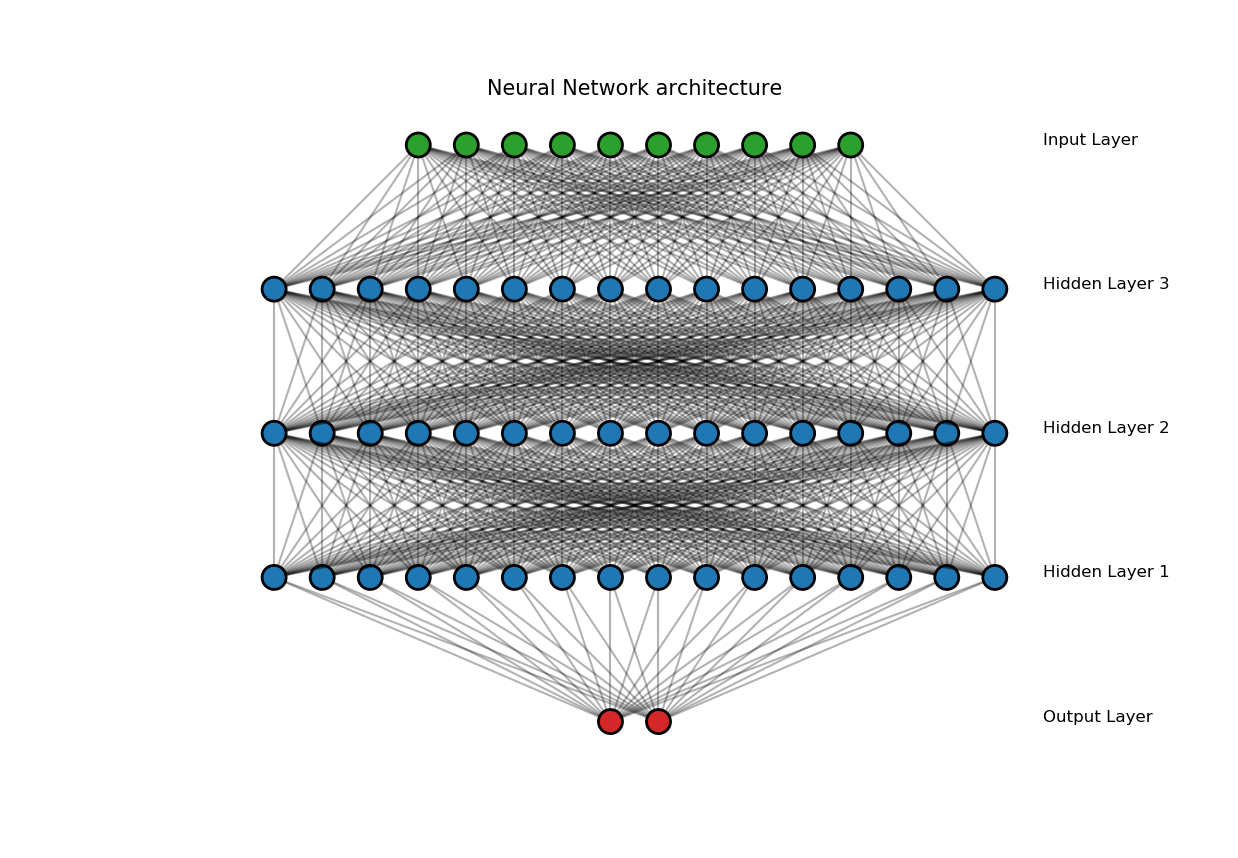
\includegraphics[width=\textwidth]{NN_NextStep_v2}
	\caption{Evaluation für die NextStep Prädiktion}
	% \todo{Quelle Bild!}
	\label{fig:boxplotErrorNNnextStep}
\end{figure}

- CV, CA
- Ergebnis Netz
- Ergebnis Lineare Regression


Vergleich Realdaten und simulierte Daten.
Realdaten mit ungefähr \SI{1.1}{\meter\per\second} während Simulierte mit \SI{1.5}{\metre\per\second} Bandgeschwindigkeit 

Zylinder schlechte performance erklären \textrightarrow orientierung fehlt

\section{Separator}

CV, CA quasi wie oben.
zusätzlich: CVBC, AA und IA

- Ergebnis NN
- Ergebnis Lineare Regression

\begin{figure}[h]
    \centering
    \missingfigure{Boxplots Result NeuralNets Separator}
	% 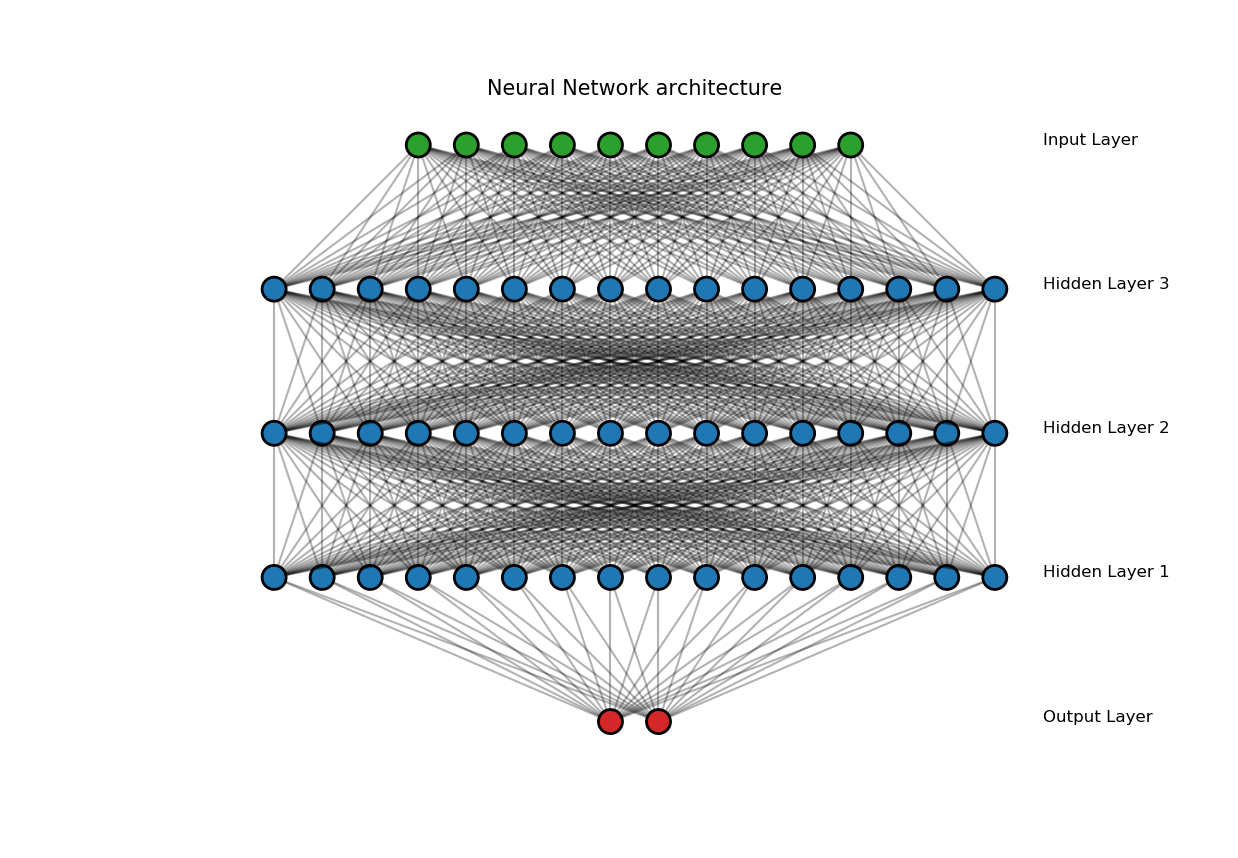
\includegraphics[width=\textwidth]{NN_NextStep_v2}
	\caption{Evaluation für die Separator Prädiktion}
	% \todo{Quelle Bild!}
	\label{fig:boxplotErrorNNSeparator}
\end{figure}